Consider a task where we attempt to predict the last word in a sentence "The clouds are in the \textit{sky}". It is fairly obvious the last word is meant to be "\textit{sky}". The gap between the relevant information and the prediction place is small, RNNs can learn to use past information and make accurate predictions. However, if we consider "I grew up in Spain... I speak fluent \textit{Spanish}", the gap between the relevant information and predicting word is large. As the gap grows, RNNs are unable to handle the task. Such problem is called \textit{long-term dependencies} \cite{colahLSTM}.

Long Short Term Memory networks (LSTM), first introduced by Hochreiter S. and Schmidhuber J. \cite{hochreiterLSTM}, are RNN architecture with the ability to handle long-term dependencies. LSTMs replace RNN's hidden states with \textbf{LSTM Cells} and add connections between cells, known as \textit{cell states} or $c_{t}$. Each LSTM Cell consists of three gates that regulate the input and output of the cell and its calculation runs as follows:

1. \textbf{Forget Gate}: Controls which information to keep and which to discard. \textit{Sigmoid function} produces a value ranging from 0 to 1 base on the information from the previous hidden state and from the current input. The value closer to 0 indicates that the information should be discarded, while a value closer to 1 means it should be kept.

\begin{equation}
    {f_t = \sigma(W_{x_f}x_t + W_{h_f}h_{t-1}+\vec{b_f})}
\end{equation}

2. \textbf{Input Gate}: Decides which information should be updated. The sigmoid function a value between 0 and 1 based on the previous hidden state and the current input state. A value close to 0 indicates unimportant information, while a value close to 1 indicates important information.

\begin{equation}
    {i_t = \sigma(W_{x_i}x_t + W_{h_i}h_{t-1}+\vec{b_i})}
\end{equation}

The information from the previous hidden state and the current input state are processed by a \textit{tanh} function, which results in values ranging from -1 to 1.

\begin{equation}
    {g_t = \tanh(W_{x_g}x_t + W_{h_g}h_{t-1}+\vec{b_g})}
\end{equation}

The decision on how to update the cell is obtained by multiplying sigmoid output and $\tanh$ output. With all the required values available, we can now calculate the \textit{cell state} as follows:

\begin{equation}
    {c_t = i_t \odot g_t + f_t \odot c_{t-1}}
\end{equation}


3. \textbf{Output Gate}: Determines what information should the next hidden state contain. The previous hidden state and the current input are passed into a sigmoid function.

\begin{equation}
    {o_t = \sigma(W_{x_o}x_t + W_{h_o}h_{t-1}+\vec{b_o})}
\end{equation}

Passing the newly modified cell state into a tanh function and multiplying its output with the sigmoid output, we get the hidden state \cite{guideLSTM}.

\begin{equation}
    {h_t = o_t \odot tanh(c_t)}
\end{equation}


The output $\hat{y}_t$ is calculated the same way as regular RNN \cite{matous}.

\begin{equation}
    {\hat{y}_t = g(W_{y}h_t + \vec{b_y})}
\end{equation}

\begin{figure}[h]
    \centering
    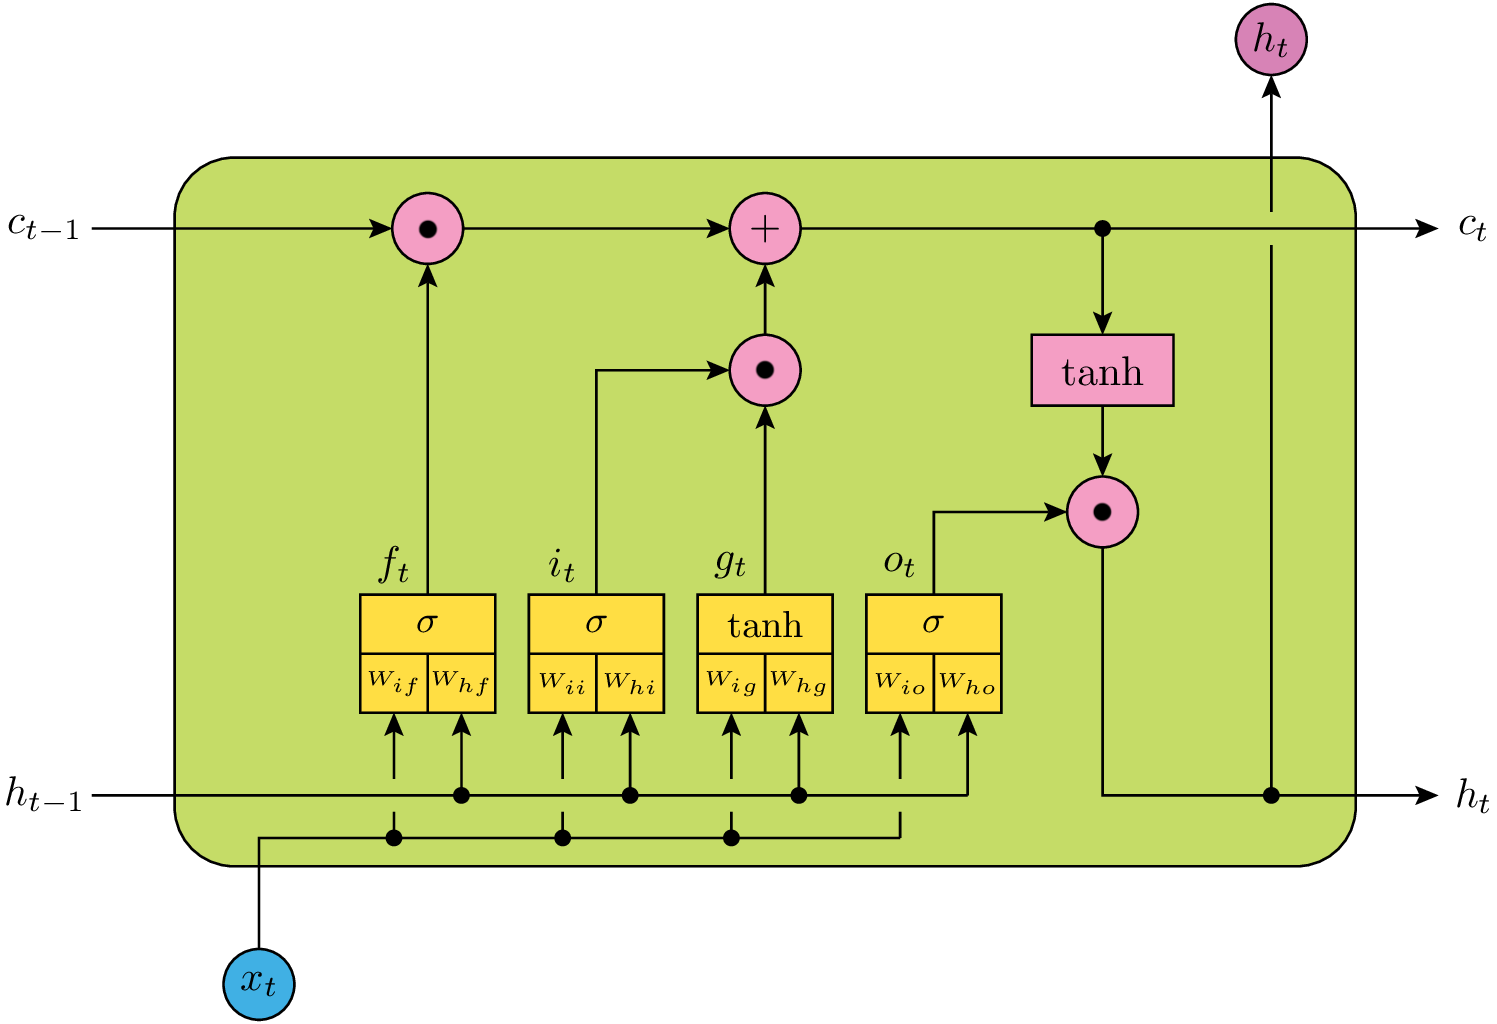
\includegraphics[width=10cm]{lstm_cell.png}
    \caption{LSTM cell \cite{lstmcell_img}}
    \label{fig:lstmCell}
\end{figure}